% Beispiel-Präsentation mit LaTeX Beamer im KIT-Design
%% entsprechend den Gestaltungsrichtlinien vom 1. August 2020
%%
%% Siehe https://sdqweb.ipd.kit.edu/wiki/Dokumentvorlagen

%% Beispiel-Präsentation
\documentclass{sdqbeamer} 
\usepackage{graphicx}
\usepackage{listings}
\usepackage{stackengine}
\graphicspath{{./slides/images}} 
%% Titelbild
\titleimage{banner_2020_kit}

%% Gruppenlogo
%\grouplogo{mylogo} 
\grouplogo{}
%% Gruppenname und Breite (Standard: 50 mm)
\groupname{Linux Internals proseminar}
%\groupnamewidth{50mm}

% Beginn der Präsentation

\title[Linux Namespaces]{Linux Namespaes}
\subtitle{KIT: Testing OS-Level Virtualization
for Functional Interference Bugs} 
\author[Jean Diestl]{Jean Diestl}

\date[6.\,6.\,2023]{6. Juni 2023}

% Literatur 
\usepackage{wrapfig}
\usepackage[citestyle=authoryear,bibstyle=numeric,hyperref,backend=biber]{biblatex}
\addbibresource{proseminar.bib}
\bibhang1em

\begin{document}
\KITtitleframe
\grouplogo{}
\section{Namespaces}
\subsection{introduction}
\begin{frame}{Container}{~}
    \begin{figure}
        \center
            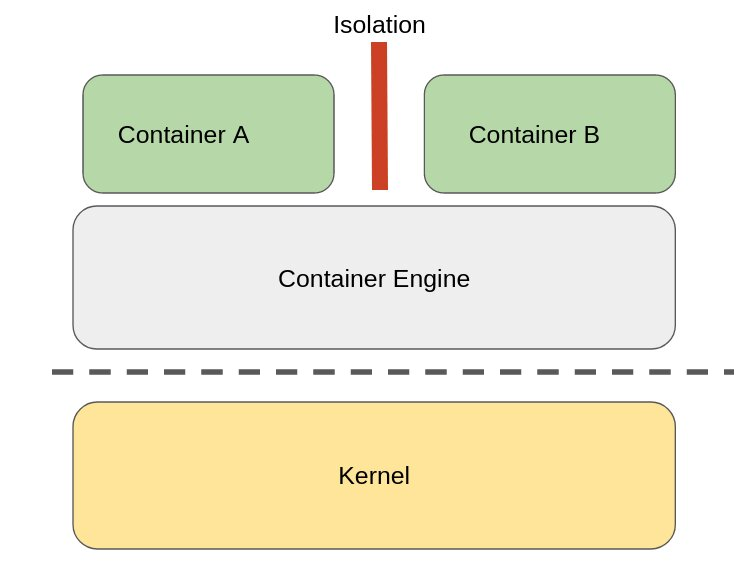
\includegraphics[scale=0.3]{/tmp/containerIntro}
        
    \end{figure}

\end{frame}
\large
\begin{frame}{Namespaces}{What are namespaces?}
\begin{minipage}{0.5\textwidth}
    

\begin{itemize}
    \setlength\itemsep{1em}
    \item process virtualization
    \item isolates global resources
    \item 7 types 
    \item management via system calls
    \item \textbf{All namespaces share the same kernel}
\end{itemize}
\end{minipage}
\hfill
\begin{minipage}{0.3\textwidth}
    \begin{greenblock}{Namespace types:}
        \begin{itemize}
            \item Mount
            \item Process ID
            \item Network
            \item IPC
            \item User ID
            \item Control group
        \item UTS
            \item time namespace
    \end{itemize}
    \end{greenblock}
\end{minipage}
\end{frame}
\subsection{simple example}
\graphicspath{{./slides/images}}
\begin{frame}{Simple example}{~}
    \begin{figure}
        
    \center
    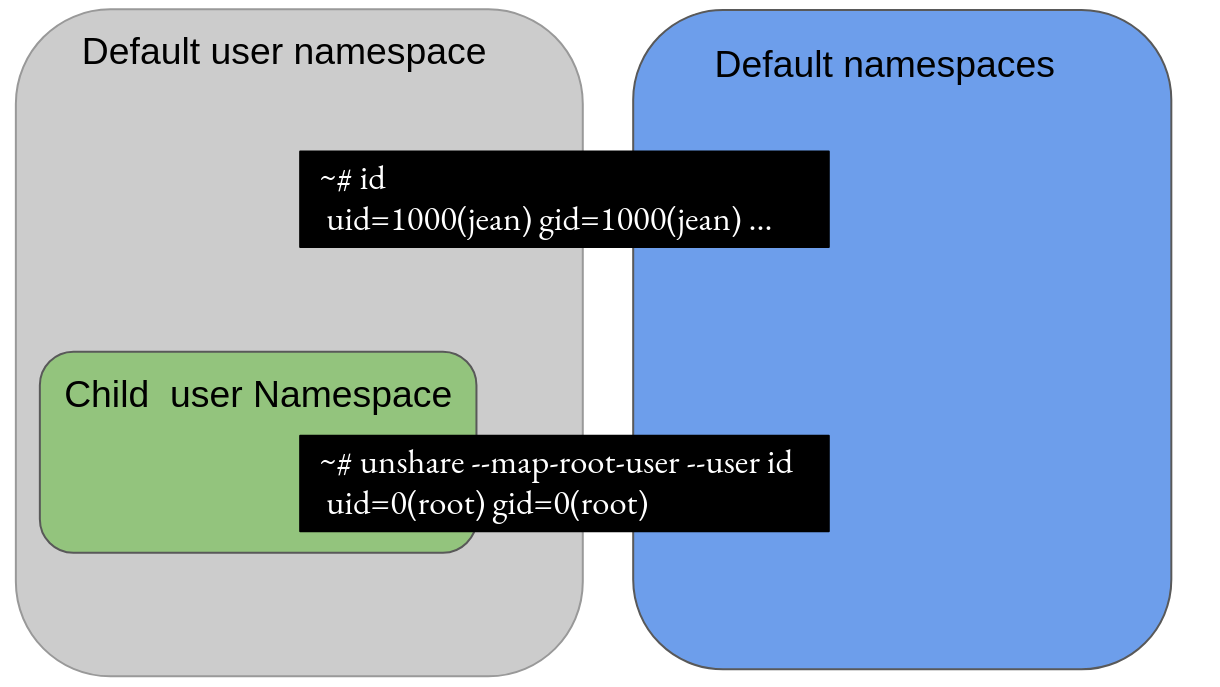
\includegraphics[scale=0.28]{/tmp/exam}
    \end{figure}
\end{frame}
\subsection{Another example}
\begin{frame}
\begin{minipage}{0.45\textwidth}

\lstinputlisting[lastline = 14,stringstyle=\color{orange},        basicstyle=\footnotesize\ttfamily,
keywordstyle=\bfseries\color{green!40!black},
commentstyle=\itshape\color{purple!40!black},
emphstyle=\bfseries\color{red},
identifierstyle=\color{blue},language=C,emph={uname,unshare,setns,clone,sethostname}]{slides/shortCode.c}
\normalsize
\texttt{[P] parent hostname demo-host\newline
[C] hostname: container\newline
[P] child hostname container\newline
[C] new hostname container2\newline
[P] child hostname container
}
\end{minipage}
\
\begin{minipage}{0.45\textwidth}

    \lstinputlisting[firstline = 15,stringstyle=\color{orange},
    emphstyle=\bfseries\color{red},
    basicstyle=\footnotesize\ttfamily,
    keywordstyle=\bfseries\color{green!40!black},
    commentstyle=\itshape\color{purple!40!black},
    identifierstyle=\color{blue},language=C,emph={uname,unshare,setns,clone,sethostname}]{slides/shortCode.c}

    \end{minipage}
%TODO
\end{frame}
%\include{slides/page2}
\section{KIT}
\subsection{Interference Bugs}
\begin{frame}{Interference Bugs}{~}
\begin{minipage}{0.4 \textwidth}
    \begin{itemize}
    \setlength\itemsep{1em}
    \item focuses on functional interference
    \item implemented in around 7500 lines of code 
    \item found 9 bugs
    \item pipeline design
\end{itemize}
\end{minipage}
\begin{minipage}{0.45\textwidth}
    \lstinputlisting[stringstyle=\color{orange},
    basicstyle=\small\ttfamily,
    keywordstyle=\bfseries\color{green!40!black},
    commentstyle=\itshape\color{purple!40!black},
    identifierstyle=\color{blue},language=C]{slides/bug_code.c}

\end{minipage}
\end{frame}

%static int ptype_seq_show(...){
%    ...
%    if (pt->dev == NULL || dev_net(pt->dev)==seq_file_net(seq)) {
%        if (pt->type == htons(ETH_P_ALL))
%            seq_puts(seq,"ALL ");
%        else
%    }
%    ...
%    }
\section{KIT}
\subsection{Interference Bugs}
\begin{frame}{KIT}{Kernel Isolation Tester}
\begin{itemize}
    \setlength\itemsep{1em}
    \item focuses on functional interference
    \item implemented in around 7500 lines of code 
    \item found 9 bugs
    \item pipeline design
\end{itemize}
\begin{figure}[hb]
    \centering
\def\stackalignment{l}
\stackunder{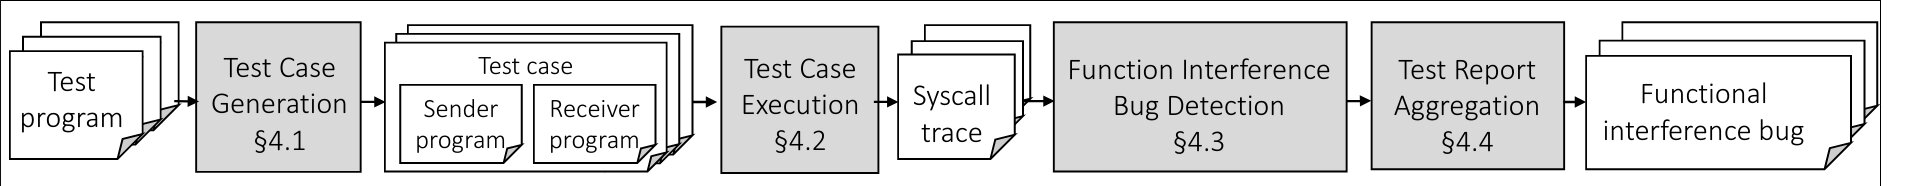
\includegraphics[scale=0.246]{/tmp/designOverview}}
           {\scriptsize
            Source: C. Liu,S. Gong and P. fonseca, KIT  Testing OS-Level Virtualization for Functional InterferenceBugs" (ASPLOS'23)}
    \end{figure}
\end{frame}
%\include{slides/howDoesKitWork}
\begin{frame}{Test case generation}{~}
\begin{itemize}
    \setlength\itemsep{1em}
    \item take test program as input
    \item find shared memory access
    \item cluster test cases to reduce load 
\end{itemize}
\begin{greenblock}{clustering}
We only need to test one test case per cluster.

\end{greenblock}

\end{frame}
\subsection{Execution}

\begin{frame}{Test case execution}{~}


\begin{minipage}{0.4 \textwidth}
    \begin{itemize}
    \setlength\itemsep{1em}
    \item system call traces and kernel stack traces are collected
    \item comapre sysetm call trees as AST
    \item limited to predictable systemcalls
\end{itemize}
\end{minipage}
\begin{minipage}{0.45\textwidth}
    \begin{figure}
        \center
    \def\stackalignment{l}
    \stackunder{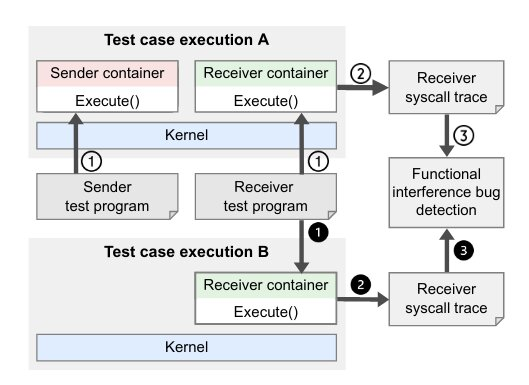
\includegraphics[scale=0.2]{/tmp/functionalInterferenceTesting}}
               {\scriptsize
                Source: C. Liu,S. Gong and P. fonseca, "KIT Testing }
                 {\scriptsize OS-Level Virtualization for Functional InterferenceBugs"(ASPLOS'23)}
    \end{figure}
\end{minipage}
\end{frame}
\subsection{report aggregation}
\begin{frame}{Test report aggregation}{~}
\begin{itemize}
    \setlength\itemsep{1em}
    \item identify system call pair that triggers bug
    \item group reports by triggering system call pair
    \item show only one report per group
\end{itemize}


\end{frame}
%\include{slides/kitPerformance}
\section{Conclusion}
\begin{frame}{Conclusion}{~}

\begin{itemize}
    \setlength\itemsep{1em}
    \item KIT is a dynamic kernel isolation test framework for system calls
    \item KIT seems to be effective
    \item KIT lacks support for system calls with dynamic output
    \item KIT only covers system call traces 
\end{itemize}


\end{frame}
%\begin{frame}{Literatur}
%\printbibliography
%\end{frame}
\end{document}